\documentclass[11pt]{article}
\usepackage[letterpaper,landscape,margin=1.5cm]{geometry}
\usepackage[T1]{fontenc}
\usepackage[utf8]{inputenc}
\usepackage{mathpazo}
\usepackage{amsmath}
\usepackage[expansion=false]{microtype}
\usepackage{xcolor}
\usepackage{colortbl}
\usepackage{multicol}
\setlength{\columnsep}{0.9cm}
\usepackage{tikz}
\usetikzlibrary{shadings,decorations.pathmorphing,decorations.markings,calc,arrows.meta,backgrounds,patterns,positioning,shapes.geometric}

% ── paleta científica sobre blanco ──────────────────────────────────
\definecolor{ink}{HTML}{1A1A1A}
\definecolor{paper}{HTML}{FFFFFF}
\definecolor{rule}{HTML}{C2C2BA}
\definecolor{virtual}{HTML}{2F5FCC}
\definecolor{vegetal}{HTML}{2F8A3E}
\definecolor{validada}{HTML}{8C8678}
\definecolor{token}{HTML}{B5851A}
\definecolor{opaque}{HTML}{6A5E9C}
\definecolor{warn}{HTML}{C0563C}

\newcommand{\tech}[1]{{\footnotesize\textls[110]{\textsc{#1}}}}
\newcommand{\noet}[1]{{\itshape #1}}
% flecha de dirección a media trayectoria
\tikzset{dir/.style={postaction={decorate},decoration={markings,
  mark=at position #1 with {\arrow[line width=0.5pt]{Stealth[length=3.6pt]}}}}}

\setlength{\parindent}{0pt}\setlength{\parskip}{0.55em}

\tikzset{
  actor/.style={draw=ink,line width=0.6pt,rounded corners=2pt,fill=paper,inner sep=4pt,align=center,font=\footnotesize},
  gate/.style={draw=opaque,line width=0.9pt,rounded corners=2pt,fill=opaque!6,inner sep=6pt,align=center,font=\footnotesize},
  ngo/.style={draw=validada,line width=0.7pt,trapezium,trapezium left angle=66,trapezium right angle=66,trapezium stretches body,minimum width=3cm,fill=validada!12,inner sep=3pt,align=center,font=\footnotesize,text=ink!72},
  ghost/.style={draw=validada!55,line width=0.6pt,dash pattern=on 1.6pt off 1.6pt,rounded corners=2pt,inner sep=3pt,align=center,font=\scriptsize,text=ink!42},
  north/.style={draw=validada,line width=0.6pt,rounded corners=2pt,fill=validada!6,inner sep=4pt,align=center,font=\footnotesize,text=ink!72},
  chain/.style={draw=vegetal,line width=0.8pt,rounded corners=2pt,fill=paper,inner sep=4pt,align=center,font=\footnotesize},
  ev/.style={font=\scriptsize\itshape,inner sep=1.5pt},
  fl/.style={-{Stealth[length=4pt]},line width=0.6pt},
  >=Stealth}

\begin{document}
\pagestyle{empty}

{\small\textls[180]{\textsc{Objeto de investigación liminal}}\hfill\textls[180]{\textsc{Módulo P · Corporación Manakai}}}
\vspace{0.1em}

{\Large\itshape El tránsito de una voz.}\\[-0.25em]
{\small\color{ink!60}La máquina de la traducción política: del aullido a la inscripción, y de la inscripción a su negativa. \textsc{\footnotesize fig. 1 — lámina} · \textsc{\footnotesize fig. 2 — detalle} · \textsc{\footnotesize fig. 3 — autómata} · \textsc{\footnotesize fig. 4 — desintermediación}}

\vspace{0.4em}

% ════════════════════════════════════════════════════════════════════
%  FIG. 1 — LÁMINA COMPLETA (blanco)
% ════════════════════════════════════════════════════════════════════
\vspace{0.6em}
\begin{center}\begin{minipage}{0.86\linewidth}\small\color{ink!85}
Las cuatro figuras componen un mismo argumento leído a cuatro escalas: la \emph{lámina} (el sistema situado en su conjunto), el \emph{detalle} (su corazón deliberativo), el \emph{autómata} (su inscripción formal) y la \emph{desintermediación} (su consecuencia política). Cada figura va precedida por una página de teoría que la guía. El método es la práctica como episteme: el diagrama no ilustra una tesis previa, la ejecuta. Y el principio rector es endofísico (Rössler, 1998): no hay vista desde afuera; quien lee está dentro del sistema que el diagrama dibuja.
\end{minipage}\end{center}

\newpage
{\Large\itshape Figura 1 · El tránsito de una voz — la máquina situada}\\[0.15em]
{\small\color{ink!60}Por qué la biocracia es una máquina de estados sin panel de control.}
\vspace{0.5em}

\begin{multicols}{2}\small\setlength{\parindent}{1em}\setlength{\parskip}{0.45em}
El proyecto no comenzó con una pregunta sino con un sonido: el aullido del \emph{Alouatta seniculus} al amanecer, en la Reserva Manakai, bosque seco tropical de Planeta Rica (Córdoba). Esa voz que convoca es el primer acto político de la biocracia, y la lámina dibuja el trayecto que recorre hasta convertirse —o negarse a convertirse— en inscripción.

La figura es una máquina de estados, pero \emph{situada}. Donna Haraway, en \emph{Situated Knowledges} (1988), mostró que todo conocimiento es parcial y encarnado: una mirada desde un cuerpo, frente al ``truco de dios'' de una objetividad sin lugar. Lucy Suchman, en \emph{Plans and Situated Actions} (1987), añadió que los planes son recursos para la acción, no su determinación —una crítica directa al modelo plan/autómata—. De ahí que esta máquina no tenga panel ni vista cenital: es un órgano dentro del sistema, no un tablero que lo gobierne desde arriba (endofísica; Rössler, \emph{Endophysics}, 1998).

El espacio de estados son las tres RV de Roy Ascott (\emph{When the Jaguar Lies Down with the Lamb}, 2001): la RV Virtual (lo digital, telemático), la RV Vegetal (lo vivo, lo opaco) y la RV Validada, la ``realidad autorizada'' que —advierte Ascott— convirtió la Naturaleza en un conjunto de objetos dispuestos en espacio euclidiano. Por eso las aristas del simplex se curvan apenas: para no repetir esa reducción. El sustrato es la \emph{moistmedia} —lo seco digital acostado con lo húmedo vivo— y la señal entre presencias viaja como biofotón, en la lectura que Jeremy Narby hace de la comunicación del ADN (\emph{La serpiente cósmica}, 1995/1998): información en forma de luz.

Se lee así: la voz entra por lo Vegetal y es \textsc{sensed} por el AudioMoth; se vuelve \textsc{present} y se desvanece en segundos; ingresa al \textsc{overlap buffer}, se adjudica y se bifurca. Dos leyes la gobiernan. La transición obedece el imperativo de Heinz von Foerster —obrar de modo que aumente el número de opciones (von Foerster, 1992)—, de suerte que el sistema se mide por lo que abre, no por lo que clausura. Y la RV Validada opera como atractor extractivo: si la voz cae hacia la cosificación, la máquina reinyecta opciones y la aparta. El anillo exterior es el reloj fenológico, tiempo lento que condiciona el sentido; el velo es la cláusula de opacidad (Glissant), una región que el diagrama se niega a representar.
\end{multicols}

\newpage
\begin{center}
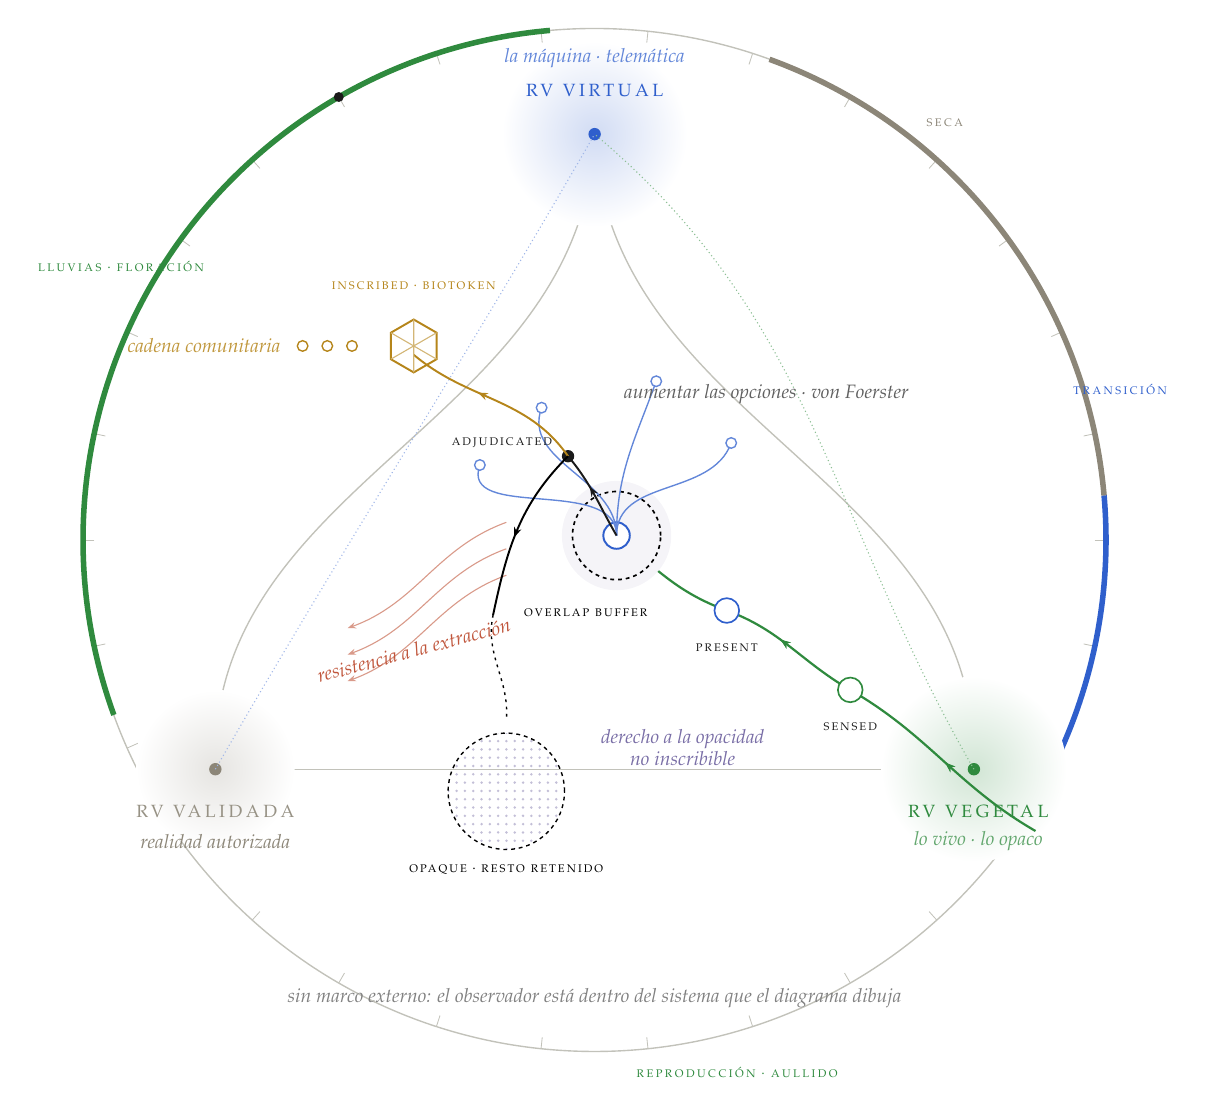
\begin{tikzpicture}[scale=1.12,every node/.style={font=\footnotesize}]

% ── anillo fenológico (reloj lento) ──────────────────────────────────
\def\Cx{8}\def\Cy{6.4}\def\Rr{5.8}
\draw[rule,line width=0.5pt] (\Cx,\Cy) circle (\Rr);
\foreach \a in {0,12,...,359}{\draw[rule,line width=0.3pt]
  ([shift=(\a:\Rr-0.13)]\Cx,\Cy)--([shift=(\a:\Rr)]\Cx,\Cy);}
\draw[vegetal, line width=2pt] ([shift=(95:\Rr)]\Cx,\Cy) arc (95:200:\Rr);
\draw[virtual, line width=2pt] ([shift=(5:\Rr)]\Cx,\Cy)  arc (5:-30:\Rr);
\draw[validada,line width=2pt] ([shift=(70:\Rr)]\Cx,\Cy) arc (70:5:\Rr);
\fill[ink] ([shift=(120:\Rr)]\Cx,\Cy) circle (1.6pt);
\node[vegetal,font=\tiny] at ([shift=(150:\Rr+0.4)]\Cx,\Cy){\textls[130]{\textsc{lluvias · floración}}};
\node[vegetal,font=\tiny] at ([shift=(285:\Rr+0.45)]\Cx,\Cy){\textls[130]{\textsc{reproducción · aullido}}};
\node[virtual,font=\tiny] at ([shift=(16:\Rr+0.4)]\Cx,\Cy){\textls[130]{\textsc{transición}}};
\node[validada,font=\tiny] at ([shift=(50:\Rr+0.38)]\Cx,\Cy){\textls[130]{\textsc{seca}}};

% ── polos · las tres RV (espacio apenas curvado) ─────────────────────
\coordinate (V) at (8,11.0);
\coordinate (G) at (12.3,3.8);
\coordinate (D) at (3.7,3.8);
\begin{scope}[rule,line width=0.5pt]
  \draw (V) to[out=-92,in=92] (D);
  \draw (V) to[out=-88,in=88] (G);
  \draw (D) -- (G);
\end{scope}
\foreach \P/\c/\rr in {V/virtual/1.05,G/vegetal/1.05,D/validada/0.9}{
  \shade[inner color=\c!22,outer color=paper] (\P) circle (\rr);
  \fill[\c] (\P) circle (2pt);}
\node[virtual]  at ($(V)+(0,0.5)$){\textls[110]{\textsc{rv virtual}}};
\node[virtual!75,font=\scriptsize\itshape] at ($(V)+(0,0.86)$){la máquina · telemática};
\node[vegetal]  at ($(G)+(0.05,-0.48)$){\textls[110]{\textsc{rv vegetal}}};
\node[vegetal!75,font=\scriptsize\itshape] at ($(G)+(0.05,-0.82)$){lo vivo · lo opaco};
\node[validada!90]at ($(D)+(0,-0.48)$){\textls[110]{\textsc{rv validada}}};
\node[validada,font=\scriptsize\itshape] at ($(D)+(0,-0.82)$){realidad autorizada};

% ── biofotones (señal-luz, Narby): tenues ───────────────────────────
\draw[vegetal!55,line width=0.4pt,densely dotted] (G) to[out=120,in=-40] (V);
\draw[virtual!45,line width=0.4pt,densely dotted] (D) to[out=60,in=240] (V);

% ── undertow → resistencia a la extracción ──────────────────────────
\foreach \i in {0,1,2}{\draw[warn!60,line width=0.4pt,-{Stealth[length=3pt]}]
  ($(7.0,6.0)+(0,0.3*\i)$) to[out=200,in=20] ($(5.2,4.8)+(0,0.3*\i)$);}
\node[warn,font=\scriptsize\itshape,rotate=15] at (5.95,5.15){resistencia a la extracción};

% ── EL TRÁNSITO ─────────────────────────────────────────────────────
\def\Path{(13.0,3.1) to[out=150,in=-30] (10.9,4.7)
          to[out=150,in=-20] (9.5,5.6) to[out=160,in=-40] (8.25,6.45)}
\draw[vegetal,line width=0.8pt,dir=0.22,dir=0.62] \Path;

\newcommand{\stnode}[4]{\fill[paper](#1,#2)circle(0.14);\draw[#3,line width=0.6pt](#1,#2)circle(0.14);
  \node[ink,font=\tiny] at (#1,#2-0.42){\textls[100]{\textsc{#4}}};}
\stnode{10.9}{4.7}{vegetal}{sensed}
\stnode{9.5}{5.6}{virtual}{present}

% Overlap Buffer (órgano de la deliberación)
\fill[opaque!7](8.25,6.45)circle(0.62);
\draw[opaque,line width=0.6pt,dash pattern=on 1.4pt off 1.4pt](8.25,6.45)circle(0.5);
\fill[paper](8.25,6.45)circle(0.15);\draw[virtual,line width=0.7pt](8.25,6.45)circle(0.15);
\node[opaque,font=\tiny] at (7.9,5.58){\textls[100]{\textsc{overlap buffer}}};
% ramificación von Foerster
\begin{scope}[virtual,line width=0.5pt]
  \foreach \x/\y in {7.4/7.9, 8.7/8.2, 6.7/7.25, 9.55/7.5}{
    \draw[virtual!75] (8.25,6.45) to[out=90,in=-110] (\x,\y);
    \fill[paper](\x,\y)circle(0.06);\draw[virtual!75,line width=0.5pt](\x,\y)circle(0.06);}
\end{scope}
\node[ink!70,font=\scriptsize\itshape] at (9.95,8.05){aumentar las opciones · von Foerster};

% Adjudicación (umbral)
\draw[ink,line width=0.7pt,dir=0.6] (8.25,6.45) to[out=120,in=-50] (7.7,7.35);
\fill[ink](7.7,7.35)circle(0.07);
\node[ink,font=\tiny] at (6.95,7.5){\textls[100]{\textsc{adjudicated}}};

% ramo A · inscripción → BioToken
\draw[token,line width=0.7pt,dir=0.6] (7.7,7.35) to[out=125,in=-40] (5.95,8.5);
\begin{scope}[shift={(5.95,8.6)}]
  \draw[token,line width=0.7pt] (90:0.3)--(150:0.3)--(210:0.3)--(270:0.3)--(330:0.3)--(30:0.3)--cycle;
  \draw[token!60,line width=0.4pt] (90:0.3)--(270:0.3) (150:0.3)--(330:0.3) (210:0.3)--(30:0.3);
\end{scope}
\node[token,font=\tiny] at (5.95,9.28){\textls[100]{\textsc{inscribed · biotoken}}};
\begin{scope}[token,line width=0.5pt]\foreach \i in {0,1,2}{\draw ($(5.25,8.6)+(-0.28*\i,0)$) circle (0.06);}\end{scope}
\node[token!85,font=\scriptsize\itshape,anchor=east] at (4.55,8.6){cadena comunitaria};

% ramo B · OPACIDAD → región deliberadamente velada (resto no inscribible)
\draw[opaque,line width=0.7pt,dir=0.55] (7.7,7.35) to[out=-135,in=78] (6.85,5.55);
\draw[opaque,line width=0.5pt,dash pattern=on 1pt off 1.6pt] (6.85,5.55) to[out=-102,in=85] (7.0,4.35);
% velo: borde punteado + trama (la trayectoria NO se dibuja dentro)
\begin{scope}
  \fill[pattern=dots,pattern color=opaque!40] (7.0,3.55) circle (0.66);
  \draw[opaque,line width=0.5pt,dash pattern=on 1.4pt off 1.4pt] (7.0,3.55) circle (0.66);
\end{scope}
\node[opaque,font=\tiny] at (7.0,2.66){\textls[100]{\textsc{opaque · resto retenido}}};
\node[opaque!90,font=\scriptsize\itshape,align=center] at (9.0,4.05){derecho a la opacidad\\ no inscribible};

% nota endofísica (sin marco externo)
\node[ink!55,font=\scriptsize\itshape] at (8,1.2){sin marco externo: el observador está dentro del sistema que el diagrama dibuja};

\end{tikzpicture}
\end{center}
\vspace{-0.1em}
{\footnotesize\color{ink!55}\textls[120]{\textsc{Fig. 1.}}\; Sustrato \noet{moistmedia} (Ascott); señal entre presencias como \noet{biofotón} (Narby). El espacio de estados son las \noet{tres RV}; sus aristas se curvan apenas, para no fijar la Naturaleza como objetos en espacio euclidiano.}

\newpage
% ════════════════════════════════════════════════════════════════════
%  FIG. 2 — DETALLE: del Overlap Buffer a la bifurcación
% ════════════════════════════════════════════════════════════════════
{\Large\itshape Figura 2 · El Overlap Buffer — el corazón deliberativo}\\[0.15em]
{\small\color{ink!60}La separación entre detectar y adjudicar, donde vive el parlamento.}
\vspace{0.5em}

\begin{multicols}{2}\small\setlength{\parindent}{1em}\setlength{\parskip}{0.45em}
El detalle amplía el único órgano donde la máquina hace verdadero trabajo de estados. Su forma proviene de la \emph{Benevolence Engine} de Bill Seaman y Otto Rössler (\emph{Neosentience: The Benevolence Engine}, 2011): una arquitectura cibernética de órganos nombrados —sensor, buffer del presente, \emph{overlap buffer}, memoria de largo plazo, motores— cuyo núcleo ético, de raíz fosteriana, sostiene que un sistema está mejor si el otro lo está. La biocracia hereda esa anatomía.

El \emph{overlap buffer} es la separación entre detección y adjudicación: simular la acción antes de ejecutarla. Una vocalización no se convierte en BioToken en el mismo instante en que se la siente; queda retenida mientras se simulan sus consecuencias. Esa retención es el parlamento. Bruno Latour había propuesto un Parlamento de las cosas (\emph{We Have Never Been Modern}, 1991; \emph{Politics of Nature}, 2004); la tesis lo extiende a lo vivo. El parlamento no vive en el disparo, sino en la demora.

Dentro del buffer, las transiciones ramifican: cada futuro simulado abre una opción más. Es la cibernética de segundo orden —la de los sistemas observantes, no sólo observados— en el linaje de las conferencias Macy, de Norbert Wiener (\emph{Cybernetics}, 1948) y Ludwig von Bertalanffy (\emph{General System Theory}, 1968), que Heinz von Foerster radicalizó (\emph{Understanding Understanding}, 2003). La deriva hacia la RV Validada —la legibilidad extractiva— se resiste activamente: la máquina reinyecta opciones y devuelve la voz al campo abierto.

Sólo entonces se bifurca. Si el evento no es opaco, cristaliza como BioToken; si la cláusula de opacidad se activa —probabilidad que crece con la cercanía a lo Vegetal y con la estación—, se retiene sin inscribirse. La adjudicación, en esta máquina, no es un veredicto que cierra sino una retención que abre: por eso su umbral se dibuja como un punto del que salen dos caminos, y no como una sentencia.
\end{multicols}

\newpage
{\large\itshape Detalle — el corazón conceptual.}\\[-0.3em]
{\small\color{ink!60}La separación entre detección y adjudicación: simular antes de ejecutar, ramificar, y bifurcar entre inscripción y retención.}

\vspace{0.6em}
\begin{center}
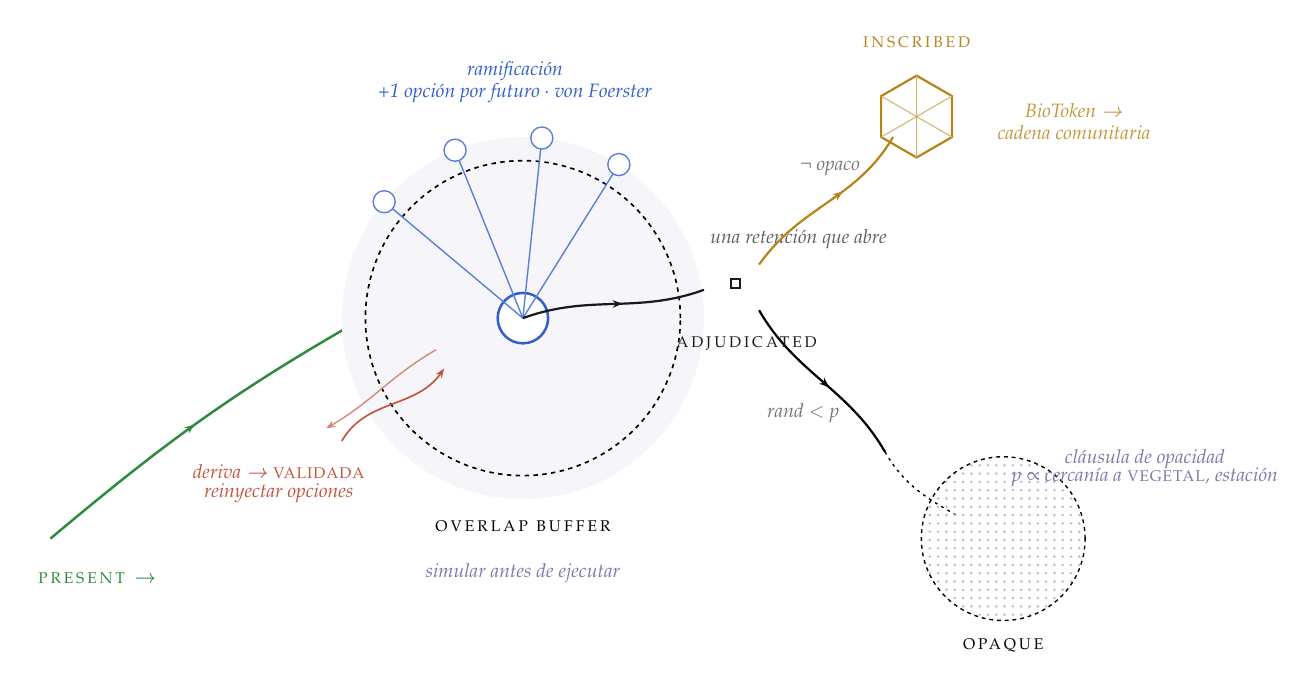
\begin{tikzpicture}[scale=2.0,every node/.style={font=\footnotesize}]

% entrada
\draw[vegetal,line width=0.9pt,dir=0.5] (-3.0,-1.4) to[out=40,in=-150] (-1.1,-0.05);
\node[vegetal,font=\scriptsize] at (-2.7,-1.65){\textls[100]{\textsc{present} →}};

% Overlap Buffer ampliado
\fill[opaque!6] (0,0) circle (1.15);
\draw[opaque,line width=0.6pt,dash pattern=on 1.6pt off 1.6pt] (0,0) circle (1.0);
\fill[paper](0,0)circle(0.16);\draw[virtual,line width=0.9pt](0,0)circle(0.16);
\node[opaque,font=\scriptsize] at (0,-1.32){\textls[110]{\textsc{overlap buffer}}};
\node[opaque!85,font=\scriptsize\itshape] at (0,-1.62){simular antes de ejecutar};

% ramas von Foerster (futuros simulados)
\foreach \ang in {58,84,112,140}{
  \draw[virtual!80,line width=0.5pt] (0,0) to[out=\ang,in=\ang-180] ([shift=(\ang:1.15)]0,0);
  \fill[paper] ([shift=(\ang:1.15)]0,0) circle (0.07);
  \draw[virtual!80,line width=0.5pt] ([shift=(\ang:1.15)]0,0) circle (0.07);}
\node[virtual,font=\scriptsize\itshape,align=center] at (-0.05,1.5){ramificación\\ \scriptsize +1 opción por futuro · von Foerster};

% deriva resistida hacia Validada
\draw[warn!70,line width=0.5pt,-{Stealth[length=3.4pt]}] (-0.55,-0.2) to[out=210,in=30] (-1.25,-0.7);
\draw[warn,line width=0.6pt,-{Stealth[length=3.4pt]}] (-1.15,-0.78) to[out=60,in=235] (-0.5,-0.32);
\node[warn,font=\scriptsize\itshape,align=center] at (-1.55,-1.05){deriva → \textsc{\scriptsize validada}\\[-0.2em]\scriptsize reinyectar opciones};

% adjudicación
\draw[ink,line width=0.8pt,dir=0.55] (0,0) to[out=20,in=200] (1.15,0.18);
\node[ink,regular polygon,regular polygon sides=4,draw,line width=0.6pt,inner sep=1.2pt,fill=paper] (adj) at (1.35,0.22){};
\node[ink,font=\scriptsize] at (1.42,-0.16){\textls[100]{\textsc{adjudicated}}};
\node[ink!70,font=\scriptsize\itshape] at (1.75,0.5){una retención que abre};

% bifurcación A: inscripción
\draw[token,line width=0.8pt,dir=0.6] (1.5,0.34) to[out=55,in=-120] (2.35,1.15);
\begin{scope}[shift={(2.5,1.28)}]
  \draw[token,line width=0.8pt](90:0.26)--(150:0.26)--(210:0.26)--(270:0.26)--(330:0.26)--(30:0.26)--cycle;
  \draw[token!60,line width=0.4pt](90:0.26)--(270:0.26)(150:0.26)--(330:0.26)(210:0.26)--(30:0.26);
\end{scope}
\node[token,font=\scriptsize] at (2.5,1.75){\textls[100]{\textsc{inscribed}}};
\node[token!85,font=\scriptsize\itshape,align=center] at (3.5,1.25){BioToken →\\ cadena comunitaria};
\node[ink!60,font=\scriptsize] at (1.95,0.95){\itshape ¬ opaco};

% bifurcación B: opacidad
\draw[opaque,line width=0.8pt,dir=0.55] (1.5,0.05) to[out=-60,in=120] (2.3,-0.85);
\draw[opaque,line width=0.5pt,dash pattern=on 1pt off 1.6pt] (2.3,-0.85) to[out=-60,in=150] (2.75,-1.25);
\begin{scope}
  \fill[pattern=dots,pattern color=opaque!45] (3.05,-1.4) circle (0.52);
  \draw[opaque,line width=0.5pt,dash pattern=on 1.4pt off 1.4pt] (3.05,-1.4) circle (0.52);
\end{scope}
\node[opaque,font=\scriptsize] at (3.05,-2.08){\textls[100]{\textsc{opaque}}};
\node[opaque!85,font=\scriptsize\itshape,align=center] at (3.95,-0.95){cláusula de opacidad\\[-0.2em] \scriptsize p $\propto$ cercanía a \textsc{vegetal}, estación};
\node[ink!60,font=\scriptsize] at (1.78,-0.6){\itshape rand $<$ p};

\end{tikzpicture}
\end{center}
{\footnotesize\color{ink!55}\textls[120]{\textsc{Fig. 2.}}\; El \noet{Overlap Buffer} es el único lugar donde la máquina hace trabajo de estados: retiene el evento, simula sus futuros (cada uno abre una opción), resiste la caída hacia lo \noet{Validado} y sólo entonces bifurca. La región velada no se dibuja por dentro: su vacío acotado \emph{es} la figura de la opacidad.}

\newpage
% ════════════════════════════════════════════════════════════════════
%  FIG. 3 — AUTÓMATA FORMAL (estados y guardas)
% ════════════════════════════════════════════════════════════════════
{\Large\itshape Figura 3 · El autómata — la inscripción rigurosa}\\[0.15em]
{\small\color{ink!60}La lectura Validada de una lámina Vegetal: el arte y la ciencia sobre una sola superficie.}
\vspace{0.5em}

\begin{multicols}{2}\small\setlength{\parindent}{1em}\setlength{\parskip}{0.45em}
El autómata es la misma máquina escrita con rigor formal: la lectura Validada de la lámina Vegetal. Una traduce a la otra sin fundirse —es lo \emph{technoético} de Ascott, techne y noesis en una sola piel—. La entrada ``State'' de Baki Cakici, en \emph{Reclaiming Technology: A Poetic-scientific Vocabulary}, mantiene tres sentidos del estado en una sola palabra: estado como materia, como polis y como máquina; la biocracia los articula a la vez. Y el ejecutable es la superficie de confluencia donde la filosofía viaja \emph{dentro} del programa, no en un texto que lo observa desde afuera: otra decisión endofísica.

Como autómata tiene estados, transiciones con guardas y dos estados terminales. Lo decisivo es que \textsc{opaque} es un estado de aceptación de pleno derecho, no un fallo: negarse a inscribir es un acto de figuración, no una omisión. Es el derecho a la opacidad de Édouard Glissant (\emph{Poética de la relación}, 1990/1997), llevado a la forma de una transición que la máquina tiene constitucionalmente prohibido completar.

Dos relojes lo gobiernan: el rápido de los eventos y el lento de la fenología, inscrito en el Módulo P y la Cámara Fenológica de lo Vivo (Arts. 41--48). Esa cámara se redacta en la forma del derecho y se lee en la forma del arte; su modelo es \emph{No Ghost Just a Shell} de Pierre Huyghe y Philippe Parreno (Annlee, 1999--2002): un acto que constituye un sujeto en lugar de describirlo. No ``da voz'' a las especies —lo que sería ventriloquia— sino que inscribe su presencia y su ausencia, medidas fenológicamente, como hechos con peso deliberativo.

El gesto se apoya en una tradición reciente del sensar ambiental. Jennifer Gabrys, en \emph{Program Earth} (2016), muestra que medir no es sólo capturar datos sino producir experiencia y formas de gobierno —la \emph{environmentality}—; y Gilbert Simondon (\emph{Du mode d'existence des objets techniques}, 1958) recuerda que el bosque mismo es ya técnico. El autómata, en consecuencia, no modela el bosque desde afuera: corre a su lado.
\end{multicols}

\newpage
{\large\itshape Autómata — la inscripción rigurosa de la máquina.}\\[-0.3em]
{\small\color{ink!60}Los mismos cinco estados como diagrama de transiciones con guardas. Es la lectura \noet{Validada} de la lámina \noet{Vegetal}: una traduce a la otra sin fundirse.}

\vspace{1.0em}
\begin{center}
\noindent\resizebox{\linewidth}{!}{%
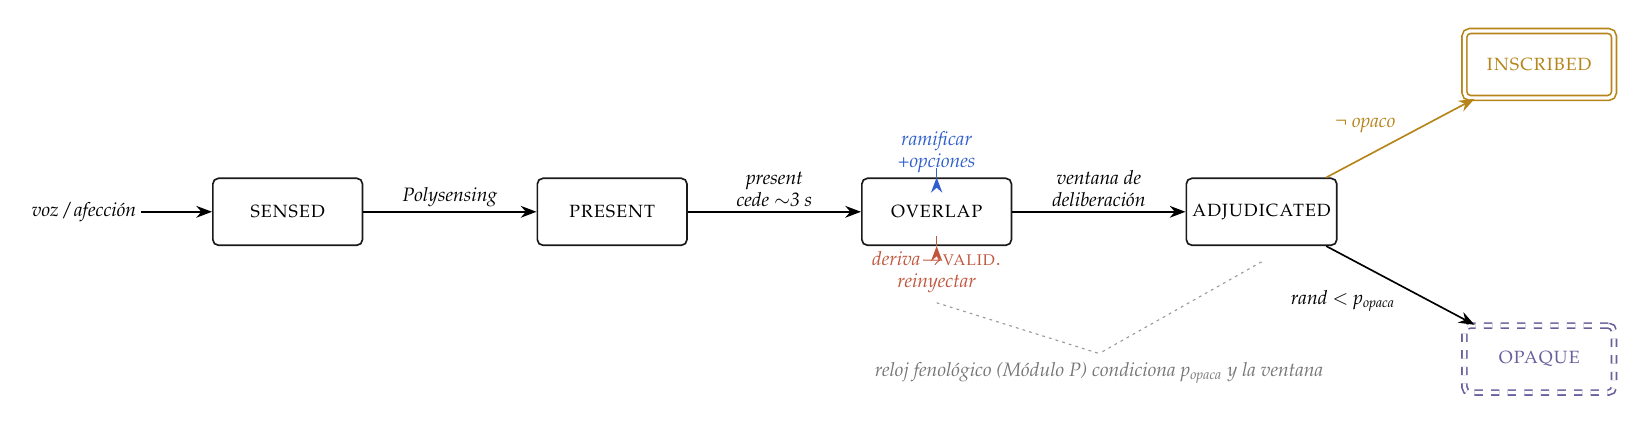
\begin{tikzpicture}[node distance=1.8cm and 2.2cm,
  st/.style={draw=ink,line width=0.6pt,rounded corners=2pt,minimum width=1.9cm,
    minimum height=0.85cm,font=\footnotesize,inner sep=2pt,align=center,fill=paper},
  term/.style={st,double,double distance=1.2pt},
  ev/.style={font=\scriptsize\itshape,inner sep=1.5pt},
  >=Stealth]

\node[st] (s) {\textsc{sensed}};
\node[st,right=of s] (p) {\textsc{present}};
\node[st,right=of p] (o) {\textsc{overlap}};
\node[st,right=of o] (a) {\textsc{adjudicated}};
\node[term,draw=token,text=token,fill=paper,above right=1.0cm and 1.6cm of a] (i) {\textsc{inscribed}};
\node[term,draw=opaque,text=opaque,fill=paper,dashed,below right=1.0cm and 1.6cm of a] (q) {\textsc{opaque}};

\draw[->,line width=0.6pt] ($(s.west)+(-0.9,0)$) node[ev,left]{voz / afección} -- (s.west);
\draw[->,line width=0.6pt] (s)--(p) node[ev,midway,above]{Polysensing};
\draw[->,line width=0.6pt] (p)--(o) node[ev,midway,above,align=center]{present\\ cede $\sim$3 s};
\draw[->,line width=0.6pt] (o)--(a) node[ev,midway,above,align=center]{ventana de\\ deliberación};
\draw[->,token,line width=0.6pt] (a)-- node[ev,above left,pos=0.5]{¬ opaco} (i);
\draw[->,opaque,line width=0.6pt] (a)-- node[ev,below left,pos=0.5]{rand $<$ p$_\text{opaca}$} (q);

\draw[->,virtual,line width=0.55pt] (o.north) to[out=120,in=60,looseness=5]
  node[ev,above,align=center,virtual]{ramificar\\ +opciones} (o.north);
\draw[->,warn,line width=0.55pt] (o.south) to[out=-120,in=-60,looseness=5]
  node[ev,below,align=center,warn]{deriva→\textsc{\scriptsize valid.}\\ reinyectar} (o.south);

\node[ink!60,font=\scriptsize\itshape,align=center] at ($(o)!0.5!(a)+(0,-2.05)$)
  {reloj fenológico (Módulo P) condiciona p$_\text{opaca}$ y la ventana};
\draw[ink!45,line width=0.4pt,dash pattern=on 1pt off 1.5pt]
  ($(o.south)+(0,-0.72)$) -- ($(o)!0.5!(a)+(0,-1.8)$);
\draw[ink!45,line width=0.4pt,dash pattern=on 1pt off 1.5pt]
  ($(a.south)+(0,-0.2)$) -- ($(o)!0.5!(a)+(0,-1.8)$);
\end{tikzpicture}}
\end{center}
{\footnotesize\color{ink!55}\textls[120]{\textsc{Fig. 3.}}\; \textsc{\footnotesize overlap} concentra las dos leyes: ramifica para \emph{abrir} (von Foerster) y resiste la deriva hacia lo \noet{Validado}. La aceptación se duplica: inscribir \emph{o} retener. \textsc{\footnotesize opaque} es un estado terminal de pleno derecho, no un fallo.}

\newpage
{\Large\itshape Figura 4 · La desintermediación — cómo se prescinde de la \textsc{\large ong}}\\[0.15em]
{\small\color{ink!60}El paso de tokenización como disolución del punto de paso obligado.}
\vspace{0.5em}

\begin{multicols}{2}\small\setlength{\parindent}{1em}\setlength{\parskip}{0.45em}
El problema que esta figura responde es el extractivismo epistémico: ONGs, universidades y agencias despliegan sensores, extraen datos y se marchan; los informes viajan al Norte Global y la comunidad de El Balzal nunca los ve. La conservación funciona, así, como una extracción encubierta: no se escucha al bosque, se extrae su legibilidad.

En esa economía, la ONG es el \emph{punto de paso obligado} —concepto de Michel Callon (\emph{Some Elements of a Sociology of Translation}, 1986) y Bruno Latour—: el cuello de botella que decide qué cuenta como verdad, quién valida y a quién se acredita el valor. La figura lo dibuja como un embudo, y lo corta.

La alternativa es la dIAP, Investigación-Acción Participativa Descentralizada, heredera de la IAP que Orlando Fals Borda formuló en Colombia (\emph{Knowledge and People's Power}, 1988): la elección de la plataforma de cadena (Algorand, Hedera, un L2 de Ethereum) no es una decisión técnica sino constitucional, deliberada en territorio. El paso de tokenización —vocalización $\rightarrow$ BioToken $\rightarrow$ cadena comunitaria de la Corporación Manakai / Parlamento de lo Vivo— reasigna las tres funciones que la ONG concentraba: ser registro de verdad pasa a la cadena, validar pasa al Parlamento, capturar el valor vuelve al territorio. El circuito extractivo es una línea abierta que sale al Norte; el biocrático, un lazo cerrado que regresa.

Conviene la advertencia: la desintermediación no la hace la cadena por sí sola —una cadena sin gobierno reproduciría la extracción con otra infraestructura—. La hacen tres cosas juntas: la cadena gobernada por el Parlamento, el retorno del valor y la cláusula de opacidad. Geoffrey Bowker, en su entrada ``Data'' de \emph{Reclaiming Technology}, recuerda que los datos son a la vez don y veneno; y Jennifer Gabrys, en \emph{Citizens of Worlds} (2022), que el sensar ciudadano sólo emancipa si no se convierte, él mismo, en una nueva máquina de legibilidad. El resto opaco que se desprende del registro es la garantía de que no lo sea.
\end{multicols}

\newpage
{\large\itshape La desintermediación — cómo se prescinde de la \textsc{\footnotesize ong}.}\\[-0.3em]
{\small\color{ink!60}El instante en que se acuña el BioToken es el instante en que la \textsc{\footnotesize ong} deja de ser el punto de paso obligado. Misma fuente, mismo sensor; dos circuitos.}

\vspace{0.4em}
\begin{center}
\resizebox{!}{11.8cm}{%
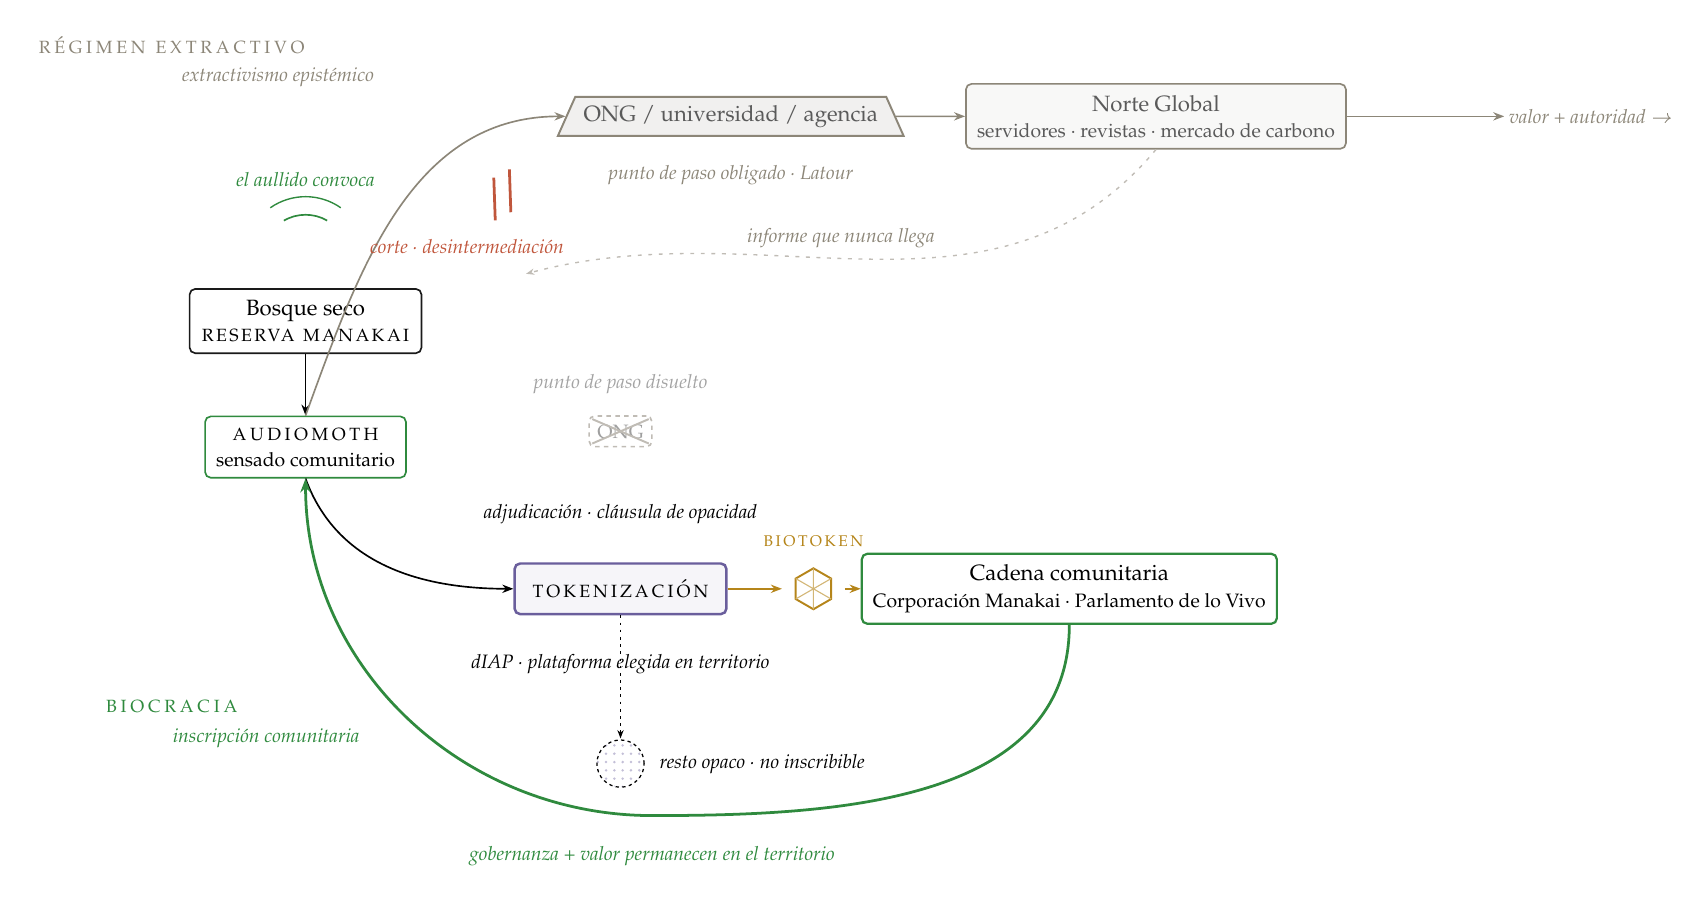
\begin{tikzpicture}[every node/.style={font=\footnotesize}]

% ── fuente común (territorio + sensor) ──────────────────────────────
\node[actor] (src) at (1.9,6.4) {Bosque seco\\ \textls[60]{\textsc{reserva manakai}}};
% glifo de aullido (la voz que convoca)
\draw[vegetal,line width=0.6pt] ([shift=(60:0.55)]1.9,7.2) arc (60:120:0.55);
\draw[vegetal,line width=0.5pt] ([shift=(55:0.78)]1.9,7.2) arc (55:125:0.78);
\node[vegetal,font=\scriptsize\itshape] at (1.9,8.2){el aullido convoca};
\node[actor,draw=vegetal] (mic) at (1.9,4.8) {\tech{audiomoth}\\ \scriptsize sensado comunitario};
\draw[fl] (src)--(mic);

% ════════════════ CIRCUITO A — régimen extractivo (gris) ════════════
\node[validada,font=\footnotesize] at (0.2,9.9) {\textls[120]{\textsc{régimen extractivo}}};
\node[validada,font=\scriptsize\itshape] at (1.55,9.5) {extractivismo epistémico};

\node[ngo] (ngo) at (7.3,9.0) {ONG / universidad / agencia};
\node[validada,font=\scriptsize\itshape] at (7.3,8.25) {punto de paso obligado · Latour};
\node[north] (north) at (12.7,9.0) {Norte Global\\ \scriptsize servidores · revistas · mercado de carbono};

\draw[fl,validada] (mic.north) to[out=70,in=180] (ngo.west);
% SEVERANCIA — la biocracia corta este enlace
\begin{scope}[shift={(4.3,7.95)},rotate=38]
  \draw[warn,line width=1pt] (-0.16,-0.22)--(0.16,0.22);
  \draw[warn,line width=1pt] (0.06,-0.26)--(0.38,0.18);
\end{scope}
\node[warn,font=\scriptsize\itshape] at (3.95,7.35) {corte · desintermediación};

\draw[fl,validada] (ngo.east)--(north.west);
\draw[fl,validada] (north.east)-- ++(2.0,0) node[ev,right,text=validada]{valor + autoridad →};
% retorno roto hacia la comunidad
\draw[validada!55,line width=0.5pt,dash pattern=on 1.4pt off 2.4pt,-{Stealth[length=3pt]}]
  (north.south) to[out=-130,in=15] (4.7,7.0);
\node[validada,font=\scriptsize\itshape] at (8.7,7.45) {informe que nunca llega};

% ════════════════ CIRCUITO B — biocracia (color vivo) ═══════════════
\node[vegetal,font=\footnotesize] at (0.2,1.5) {\textls[120]{\textsc{biocracia}}};
\node[vegetal,font=\scriptsize\itshape] at (1.4,1.1) {inscripción comunitaria};

% ONG fantasma: ya no es punto de paso
\node[ghost] (ongx) at (5.9,5.0) {ONG};
\draw[validada!55,line width=0.7pt] ($(ongx.south west)+(0.05,0.05)$)--($(ongx.north east)+(-0.05,-0.05)$);
\draw[validada!55,line width=0.7pt] ($(ongx.north west)+(0.05,-0.05)$)--($(ongx.south east)+(-0.05,0.05)$);
\node[ink!40,font=\scriptsize\itshape] at (5.9,5.6) {punto de paso disuelto};

\node[gate] (gate) at (5.9,3.0) {\textls[90]{\textsc{tokenización}}};
\node[opaque,font=\scriptsize\itshape] at (5.9,3.95) {adjudicación · cláusula de opacidad};
\node[opaque,font=\scriptsize\itshape] at (5.9,2.05) {dIAP · plataforma elegida en territorio};

% BioToken (cristal) y cadena comunitaria
\begin{scope}[shift={(8.35,3.0)}]
  \draw[token,line width=0.7pt] (90:0.26)--(150:0.26)--(210:0.26)--(270:0.26)--(330:0.26)--(30:0.26)--cycle;
  \draw[token!60,line width=0.4pt] (90:0.26)--(270:0.26)(150:0.26)--(330:0.26)(210:0.26)--(30:0.26);
\end{scope}
\node[token,font=\scriptsize] at (8.35,3.6){\textls[80]{\textsc{biotoken}}};
\node[chain] (chain) at (11.6,3.0) {Cadena comunitaria\\ \scriptsize Corporación Manakai · Parlamento de lo Vivo};

\draw[fl] (mic.south) to[out=-70,in=180] (gate.west);
\draw[fl,token] (gate.east)--(7.95,3.0);
\draw[fl,token] (8.75,3.0)--(chain.west);

% resto opaco que se desprende (no se tokeniza)
\draw[opaque,line width=0.6pt,dash pattern=on 1pt off 1.6pt,-{Stealth[length=3pt]}] (gate.south)--(5.9,1.1);
\fill[pattern=dots,pattern color=opaque!40] (5.9,0.78) circle (0.3);
\draw[opaque,line width=0.45pt,dash pattern=on 1.2pt off 1.2pt] (5.9,0.78) circle (0.3);
\node[opaque,font=\scriptsize\itshape] at (7.7,0.78) {resto opaco · no inscribible};

% RETORNO: gobernanza + valor permanecen (lazo cerrado)
\draw[vegetal,line width=1pt,-{Stealth[length=5pt]}]
  (chain.south) to[out=-90,in=0] (6.3,0.12) to[out=180,in=-90] (mic.south);
\node[vegetal,font=\scriptsize\itshape] at (6.3,-0.4) {gobernanza + valor permanecen en el territorio};

% (la reasignación de funciones se explica en el pie de figura)

\end{tikzpicture}}
\end{center}

\vspace{0.2em}
{\footnotesize\color{ink!60}\textls[120]{\textsc{Fig. 4.}}\; El paso de tokenización es donde la máquina deja de necesitar a la \textsc{\footnotesize ong}: al acuñar el \noet{BioToken} sobre una cadena gobernada por el Parlamento, las tres funciones que la \textsc{\footnotesize ong} concentraba —ser registro de verdad, validar, capturar el valor— se redistribuyen en el territorio. El circuito extractivo es una línea abierta que sale al Norte; el biocrático es un \noet{lazo cerrado} que vuelve.

\smallskip
\textit{Advertencia, contra el solucionismo de cadena:} la desintermediación no la hace la cadena por sí sola —una cadena sin gobierno reproduciría la extracción con otra infraestructura—. La hacen tres cosas juntas: la cadena \emph{gobernada por el Parlamento} (\textsc{\footnotesize dIAP}, elección constitucional de plataforma en territorio), el \emph{retorno} de valor y gobernanza, y la \emph{cláusula de opacidad}, que mantiene un resto sin inscribir para que el registro no se vuelva, él mismo, una nueva máquina de legibilidad extractiva.}

\newpage
% ── concepto ↔ técnica ──────────────────────────────────────────────
\vspace{1.4em}
{\large\itshape Los enlaces — concepto y técnica sobre una sola superficie.}

\newcommand{\lk}[3]{\noet{#1} & \tech{#2} & {\footnotesize\color{ink!65}#3}\\[0.32em]}
\begin{center}\small
\begin{tabular}{@{}p{4.4cm}@{\hskip 0.5cm}p{4.6cm}@{\hskip 0.5cm}p{5.2cm}@{}}
\textls[110]{\textsc{\footnotesize concepto}} & \textls[110]{\textsc{\footnotesize correlato técnico}} & \textls[110]{\textsc{\footnotesize procedencia}}\\[0.15em]
\arrayrulecolor{rule}\hline\\[-0.6em]
\lk{lo sentido · Polysensing}{AudioMoth · ecoacústica}{Seaman \& Rössler · Manakai}
\lk{el presente que cede}{buffer $\sim$3 s}{Benevolence Engine}
\lk{simular antes de ejecutar}{Overlap Buffer}{detección\,/\,adjudicación}
\lk{aumentar las opciones}{ramificación de transiciones}{von Foerster}
\lk{inscripción}{BioToken · cadena (dIAP)}{Latour · Parlamento de lo Vivo}
\lk{derecho a la opacidad}{resto no inscribible · velo}{Glissant}
\lk{reloj lento · fenología}{Módulo P · Arts. 41--48}{Cámara Fenológica de lo Vivo}
\lk{el motor es sonido}{OSC \texttt{/soneth/} $\rightarrow$ SuperCollider}{Lampsacus · Rössler}
\end{tabular}
\end{center}

% ── disclaimer (versión clara, con regla lateral) ───────────────────
\vspace{0.6em}
\noindent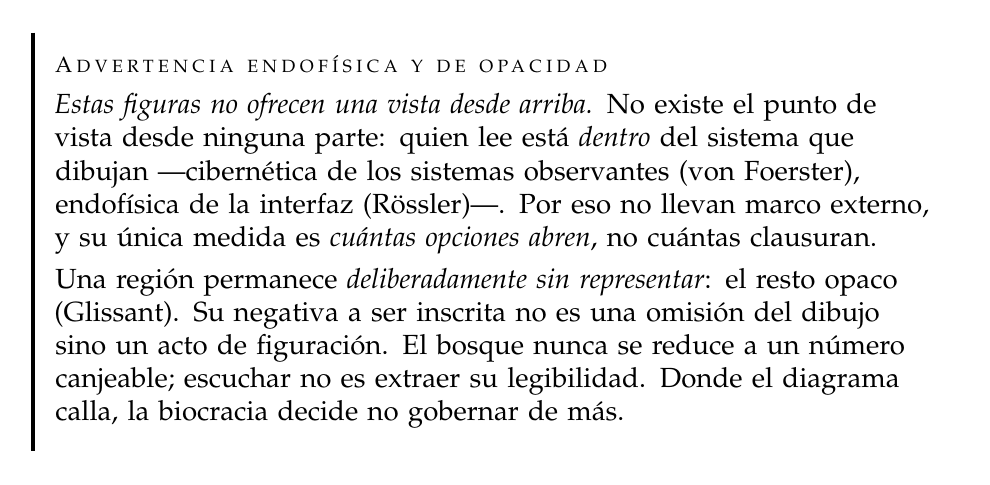
\begin{tikzpicture}
\node[inner sep=10pt,align=left,text width=0.92\linewidth] (b){%
{\textls[150]{\textsc{\footnotesize Advertencia endofísica y de opacidad}}}\\[0.3em]
{\itshape Estas figuras no ofrecen una vista desde arriba.} No existe el punto de vista desde ninguna parte: quien lee está \emph{dentro} del sistema que dibujan —cibernética de los sistemas observantes (von Foerster), endofísica de la interfaz (Rössler)—. Por eso no llevan marco externo, y su única medida es \emph{cuántas opciones abren}, no cuántas clausuran.\\[0.3em]
Una región permanece \emph{deliberadamente sin representar}: el resto opaco (Glissant). Su negativa a ser inscrita no es una omisión del dibujo sino un acto de figuración. El bosque nunca se reduce a un número canjeable; escuchar no es extraer su legibilidad. Donde el diagrama calla, la biocracia decide no gobernar de más.};
\draw[opaque,line width=1.4pt] ($(b.north west)+(2pt,-2pt)$)--($(b.south west)+(2pt,2pt)$);
\end{tikzpicture}

\newpage
{\Large\itshape Referencias citadas}\\[0.15em]
{\small\color{ink!60}Las ediciones y años se alinean con la bibliografía de la tesis; verifíquense allí.}
\vspace{0.6em}

\begin{multicols}{2}\footnotesize\setlength{\parindent}{-1em}\setlength{\leftskip}{1em}\setlength{\parskip}{0.4em}
Agamben, G. (1990/1996). \emph{La comunidad que viene}. Pre-Textos.\par
Ascott, R. (2001). When the Jaguar Lies Down with the Lamb: Speculations on the Post-biological Culture. \emph{Artnodes}, UOC.\par
Bertalanffy, L. von (1968). \emph{General System Theory}. Braziller.\par
Bowker, G. C. ``Data''. En \emph{Reclaiming Technology: A Poetic-scientific Vocabulary}.\par
Cakici, B. ``State''. En \emph{Reclaiming Technology: A Poetic-scientific Vocabulary}.\par
Callon, M. (1986). Some Elements of a Sociology of Translation. En J. Law (ed.), \emph{Power, Action and Belief}.\par
Fals Borda, O. (1988). \emph{Knowledge and People's Power}. Indian Social Institute.\par
Foerster, H. von (1992). Ethics and Second-Order Cybernetics. \emph{Cybernetics \& Human Knowing}.\par
Foerster, H. von (2003). \emph{Understanding Understanding}. Springer.\par
Gabrys, J. (2016). \emph{Program Earth: Environmental Sensing Technology and the Making of a Computational Planet}. Univ. of Minnesota Press.\par
Gabrys, J. (2022). \emph{Citizens of Worlds: Open-Air Toolkits for Environmental Struggle}. Univ. of Minnesota Press.\par
Glissant, É. (1990/1997). \emph{Poetics of Relation}. Univ. of Michigan Press.\par
Haraway, D. (1988). Situated Knowledges. \emph{Feminist Studies}, 14(3).\par
Huyghe, P. \& Parreno, P. (1999--2002). \emph{No Ghost Just a Shell}.\par
Latour, B. (1991). \emph{We Have Never Been Modern}. Harvard Univ. Press.\par
Latour, B. (2004). \emph{Politics of Nature}. Harvard Univ. Press.\par
Narby, J. (1995/1998). \emph{The Cosmic Serpent: DNA and the Origins of Knowledge}. Tarcher/Putnam.\par
Oliveros, P. (2005). \emph{Deep Listening: A Composer's Sound Practice}. iUniverse.\par
Rössler, O. (1998). \emph{Endophysics: The World as an Interface}. World Scientific.\par
Seaman, B. \& Rössler, O. (2011). \emph{Neosentience: The Benevolence Engine}. Intellect.\par
Simondon, G. (1958). \emph{Du mode d'existence des objets techniques}. Aubier.\par
Suchman, L. (1987). \emph{Plans and Situated Actions}. Cambridge Univ. Press.\par
Wiener, N. (1948). \emph{Cybernetics}. MIT Press.\par
\end{multicols}

\end{document}
